% ****** Start of file apssamp.tex ******
%
%   This file is part of the APS files in the REVTeX 4.2 distribution.
%   Version 4.2a of REVTeX, December 2014
%
%   Copyright (c) 2014 The American Physical Society.
%
%   See the REVTeX 4 README file for restrictions and more information.
%
% TeX'ing this file requires that you have AMS-LaTeX 2.0 installed
% as well as the rest of the prerequisites for REVTeX 4.2
%
% See the REVTeX 4 README file
% It also requires running BibTeX. The commands are as follows:
%
%  1)  latex apssamp.tex
%  2)  bibtex apssamp
%  3)  latex apssamp.tex
%  4)  latex apssamp.tex
%
\documentclass[%
 reprint,
%superscriptaddress,
%groupedaddress,
%unsortedaddress,
%runinaddress,
%frontmatterverbose,
%preprint,
%preprintnumbers,
%nofootinbib,
%nobibnotes,
%bibnotes,
 amsmath,amssymb,
 aps,
%pra,
prb,
%rmp,
%prstab,
%prstper,
%floatfix,
]{revtex4-2}

\usepackage{graphicx}% Include figure files
\usepackage{dcolumn}% Align table columns on decimal point
\usepackage{bm}% bold math
\usepackage{amsfonts}
\usepackage{amsmath}
\usepackage{physics}
\usepackage{amssymb}
\usepackage{mathtools}
%\usepackage{hyperref}% add hypertext capabilities
%\usepackage[mathlines]{lineno}% Enable numbering of text and display math
%\linenumbers\relax % Commence numbering lines

%\usepackage[showframe,%Uncomment any one of the following lines to test
%%scale=0.7, marginratio={1:1, 2:3}, ignoreall,% default settings
%%text={7in,10in},centering,
%%margin=1.5in,
%%total={6.5in,8.75in}, top=1.2in, left=0.9in, includefoot,
%%height=10in,a5paper,hmargin={3cm,0.8in},
%]{geometry}

\begin{document}

\preprint{APS/123-QED}

\title{Floquet-Drude Conductivity in Dressed Quantum Hall Systems}% Force line breaks with \\
% \thanks{A footnote to the article title}%

\author{Kosala Herath,}
 % \altaffiliation[Also at ]{Physics Department, XYZ University.}%Lines break automatically or can be forced with \\
\author{Malin Premaratne}%
\affiliation{%
 Advanced Computing and Simulation Laboratory(A$\chi$L), Department of Electrical and Computer Systems Engineering,\\
 Monash University, Clayton, Victoria 3800, Australia
}%

% \collaboration{MUSO Collaboration}%\noaffiliation
%
% \author{Charlie Author}
%  \homepage{http://www.Second.institution.edu/~Charlie.Author}
% \affiliation{
%  Second institution and/or address\\
%  This line break forced% with \\
% }%
% \affiliation{
%  Third institution, the second for Charlie Author
% }%
% \author{Delta Author}
% \affiliation{%
%  Authors' institution and/or address\\
%  This line break forced with \textbackslash\textbackslash
% }%
%
% \collaboration{CLEO Collaboration}%\noaffiliation

\date{\today}% It is always \today, today,
             %  but any date may be explicitly specified

\begin{abstract}
A generalized mathematical model for the transport properties of systems exposed to a stationary magnetic and a strong electromagnetic field is presented. The new formulation, which applies to the two-dimensional dressed quantum Hall systems, is based on Landau quantization theory and Floquet-Drude conductivity method. We model our system as a two-dimensional electron gas (2DEG) that interacts with two external fields. To incorporate the strong light coupling with the 2DEG, we utilize the Floquet theory to analyze the effect non perturbatively. Moreover, the Floquet Fermi "golden rule" is adopted to explore the scattering effects for Floquet states in disordered quantum Hall systems. Based on our fully analytical expression and particular graphical representations, we demonstrate
that the characteristics of conductivities in two-dimensional quantum Hall systems can manipulate using a dressed field. The outcomes align with theoretical descriptions which are already well-suited with experimental results at the same time our theory provides a more generalized analysis on the properties of conductivity in quantum Hall systems. Thus, this model more realistically describes that how to use external strong radiation as a tool to utilize transport properties in various 2D nanostructures which serve as a basis for nano-optoelectronic devices.

% \begin{description}
% \item[Usage]
% Secondary publications and information retrieval purposes.
% \item[Structure]
% You may use the \texttt{description} environment to structure your abstract;
% use the optional argument of the \verb+\item+ command to give the category of each item.
% \end{description}
\end{abstract}

%\keywords{Suggested keywords}%Use showkeys class option if keyword
                              %display desired
\maketitle

%\tableofcontents

\section{\label{sec:introduction} Introduction}
% Section 01 - Introduction

Manipulating light-matter interactions in the quantum regime paved the path for an astonishing number of useful technologies in the last century. Quantum optics, which study these interactions, have drawn research attention to the disciplines of optoelectronics \cite{liu16,wijesekara20,tao21,wijesekara21}, sensing \cite{rodrigo2015,pirandola18,hapuarachchi2018}, energy harvesting \cite{yuan16,sun18},
quantum computing \cite{huh15,slussarenko19,andersen21}, bio-information \cite{marais18,bian20}, and many other specialities of recent technologies \cite{rivera20}.
The studies on quantum optics of nanostructures were generally centered on metamaterials \cite{shalaev07,si14}, quantum plasmonic effects \cite{hapuarachchi19,perera20}, lasers and amplifiers \cite{zhang05,chow13}, and quantum cavity physics \cite{tsang10,devi20}.
However, in recent years, one of the foremost aim of examining nanostructures under external radiation was understanding their electron transport characteristics \cite{kitagawa11,zhou11,kibis14,pervishko15,morina15,dehghani15,dini16,wackerl20}.

Better understanding the fundamental mechanisms of charge transport can allow us to invent novel nanoelectronic devices and optimize their performance \cite{premaratne21}.
Most recent studies on the subject have considered the driving field as a perturbation field \cite{pervishko15,morina15}. However, this assumption breaks down for systems under high-intensity illuminations \cite{grifoni98,wackerl20}.
Modeling an electromagnetic field under a perturbative formalism involves expanding the interaction terms in powers of the field intensity. At high intensities, the higher-order terms influence the physics more strongly and the basis of the perturbative treatment begins to break down.
In these instances, a more accurate treatment needs to be adopted. Thus, we treat the interacting fermion system and the radiation as one combined quantum system, namely dressed system \cite{morina15,cohen98,scully01}. Here the applied high-intensity  electromagnetic field identify as the dressing field.

Theoretical analyses on the transport properties of dressed fermion systems were recently reported in Refs. \cite{kibis14,morina15,wackerl20}.
Furthermore, in Ref. \cite{wackerl20} a general expression for conductivity in a dressed system has been derived in a fully closed analytical form. In their study, a novel type of Green’s functions, namely four-times Green’s functions were used to derive the Floquet-Drude conductivity formula. This opened the path to exploring and exploiting nanostructures' charge transport attributes under an intense dressing field.

Quantum Hall effect \cite{girvin90} observed in two-dimensional (2D) fermion systems at low temperatures under strong stationary magnetic fields manifest remarkable magneto-transport behaviors. Transport properties of these systems have recently attracted both theoretical \cite{ando72,ando74_1,ando74_2,ando74_3,ando74_4,ando82,endo09} and experimental \cite{allerman95,tieke97,pan05} interest.
Endo \textit{et al.} \cite{endo09} presented the calculations of longitudinal and transverse conductivity tensor components and their relationship in a quantum Hall system. These theoretical calculations  align better with experimental observations compared to previous studies.

In contrast, more exciting phenomena can be observed by simultaneously applying a dressing field to a quantum Hall system already under a non-oscillating magnetic field.
Whilst there exist several leading theories for calculating conductivity tensor elements in quantum Hall systems \cite{ando74_1,ando82,endo09}, they have not been utilized to describe the optical manipulation of charge transport.
Recently, Dini \textit{et al.} \cite{dini16} have investigated the one-directional conductivity behavior of dressed quantum Hall systems. However, they have not adopted the state-of-the-art model to describe the conductivity in a quantum Hall system. In their study, they used the conductivity models from Refs. \cite{ando74_1,ando82}, and as mentioned in Endo \textit{et al.} \cite{endo09}, those models predict a semi-elliptical broadening against Fermi level for each Landau level and provide less agreement with the empirical results.

In the present analysis, we present a robust mathematical model for a dressed two-dimensional electron gas (2DEG) subject to another nonoscillating magnetic field.
A stationary magnetic field is applied perpendicularly across the surface of the 2DEG system. This causes the orbital motion of the electrons to be quantized, and a discrete energy spectrum with Landau splitting is observed \cite{landau30}.
In this study, we explicitly calculate the longitudinal components ($\sigma^{xx},\sigma^{yy}$) of the conductivity tensor in a periodically driven quantum Hall system by developing a generalized analytical description using the Floquet-Drude conductivity \cite{wackerl20}.
Finally, we demonstrate that our generalized model reproduces the results of the state-of-the-art conductivity model in Ref. \cite{endo09}, which was developed for the more specific case of quantum Hall systems without the external dressing field.
Moreover, we find that the optical field can be used as a mechanism to regulate transport behavior in numerous 2D nanostructures which can serve as a basis for many useful nanoelectronic devices. We believe that our theoretical analysis and visual depictions of numerical results will lead to a better understanding of manipulating charge transport. Moreover, this will inspire advanced  developments in nanoscale quantum devices.

The paper is organized as follows. Sec.  \ref{sec_schrodinger_problem} introduces our dressed quantum Hall system and the exact wave function solutions for the given configuration. Sec. \ref{sec_floquet_theory} provides the Floquet theory interpretation of these wave functions.
We introduce Floquet-Fermi golden rule for a quantum Hall system in Sec. \ref{sec_inverse_scattering_time}, and use it in Sec. \ref{sec_floquet_drude_conductivity} to derive analytical expressions for longitudinal components of conductivity.
The derived theoretical model is further analyzed numerically using empirical system parameters and compared with previous studies in Sec. \ref{sec_manipulate_conductivity}.
In Sec. \ref{sec_conclusions}, we summarize our analysis and present our conclusions.


\section{Schrödinger problem for Landau levels in dressed 2DEG
}
% Section 02 - Schrodinger problem for dressed quantum Hall system

Our system consist of a two-dimentional free electron gas (2DEG) confined in the $(x,y)$ plane of the three-dimentional coordinate space. In our analysis, the 2DEG is subjected to a stationary magnetic field $\vb{B} = (0,0,B)^{\text{T}}$ which is pointed towards the $z$ axis. In addition, a linearly polarized strong light is applied perpendicular to the 2DEG plane, and we specially tune the frequency of the field $\omega$ such that the optical field behaves as a purely dressing field (unabsorbable). Without limiting the generality we can choose $y$-polorized electric field $\vb{E} = (0,E\sin(\omega t),0)^{\text{T}}$ for the dressing field configuration (Fig.~\ref{fig_1}).
\begin{figure}[b]
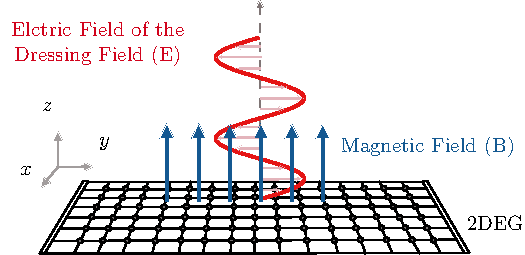
\includegraphics[scale=0.9]{figures/fig_1}
\caption{\label{fig_1} Two-dimensional electron gas (2DEG) confined in the $(x,y)$ plane while both stationary magnetic field $\vb{B}$ and strong dressing field with y-polarized electric field $\vb{E}$ are being applied perpendicular to the surface of 2DEG.}
\end{figure}
Here $B$ and $E$ represent the amplitude of the stationary magnetic field and oscillating electric field respectively.

Using Landau gauge for the stationary magnetic field, we can represent it using vector potential as $\vb{A}_{s} = (-By,0,0)^{\text{T}}$ and choosing Coulomb gauge, the vector potential of the dynamic dressing radiation can be presented as $\vb{A}_{d}(t) = (0,[E/\omega ]\cos(\omega t),0)^{\text{T}}$. These vector potentials are coupled to the momentum of 2DEG as kinetic momentum \cite{mahan00,bruus04} and this leads to the time-dependent Hamiltonian
\begin{equation} \label{eq_1}
  \hat{H}_e(t) = \frac{1}{2m_e}\Big[\hat{\vb{p}} - e\big(\vb{A}_{s}+\vb{A}_{d}(t)\big)\Big]^2,
\end{equation}
where $m_e$ is the effective electron mass and $e$ is the magnitude of the electron charge. $\hat{\vb{p}} = (\hat{p}_x,\hat{p}_y,0)^{\text{T}}$ represents the canonical momentum operator for 2DEG with electron momentum $p_{x,y}$.
The exact solutions for the time-dependent Schrödinger equation $i\hbar \dv{t}\psi = \hat{H}_e(t) \psi$ was already given by Refs. \cite{husmi53,ditt98,dini16} and we can present them as a set of wave functions defined by two quantum numbers $(n,m)$
\begin{equation} \label{eq_2}
  \begin{aligned}
    \psi_{n,m}&(x,y,t)  \\
    & = \frac{1}{\sqrt{L_x}}
    \chi_n\left[y - y_0 - \zeta(t)\right]\\
    & \times
    \text{exp}\bigg(
    \frac{i}{\hbar}\bigg[- \varepsilon_nt
    + p_x x + \frac{eE(y - y_0)}{\omega}\cos(\omega t)\\
    &+
    m_e\dot{\zeta}(t)\big[y - y_0 -\zeta(t)\big] +
    \int_0^{t}dt'L(\zeta,\dot{\zeta},t')\bigg]\bigg),
  \end{aligned}
\end{equation}
where $n \in \mathbb{Z}^{+}_0$ and $m \in \mathbb{Z}$ ; see Appendix A. Here $L_{x,y}$ are dimension of the 2DEG surface, $\hbar$ is the reduced Planck constant, and $y_0 = -p_x/eB$ is the center of the cyclotron orbit along $y$ axis. $\chi_n$ are well known solutions for Schrödinger equation of a stationary quantum harmonic oscillator
\begin{equation} \label{eq_3}
  \chi_n(x) \equiv
   \frac{\sqrt{\kappa}}{\sqrt{2^{n}n!}}
  e^{-\kappa^2 x^2/2}
  \mathcal{H}_n \qty(\kappa x) \quad \text{with}
  \quad
  \kappa = \sqrt{\frac{m_e \omega_0}{\hbar}},
\end{equation}
with eigenvalues given by $\varepsilon_n = \hbar \omega_0 (n + 1/2)$ and $\omega_0 = eB/m_e$ is the cyclotron frequency. Each $n$ value defines the  energy($\varepsilon_n$) of the respective Landau level. The path shift of the driven classical oscillator $\zeta(t)$ is given by
\begin{equation} \label{eq_4}
  \zeta(t) = \frac{eE}{m_e(\omega_0^2 - \omega^2)}\sin(\omega t),
\end{equation}
while the Lagrangian of the classical oscillator $L(\zeta,\dot{\zeta},t)$ can be identified as
\begin{equation} \label{eq_5}
  L(\zeta,\dot{\zeta},t) = \frac{1}{2} m_e\dot{\zeta}^2(t) - \frac{1}{2}m_e\omega_0^2 \zeta^2(t) + eE\zeta(t) \sin(\omega t).
\end{equation}
The exponential phase shifts in Eq.~(\ref{eq_2}) represent the influence done by the stationary magnetic field and strong dressing field. Therefore, we can accept that magneto-transport properties of 2DEG will be renormalized by the magnetic field as well as the dressing field.


\section{Floquet theory}
Considerable research effort in recent years has been de- voted to synthesizing materials whose thermal conductivity.


\section{Floquet Fermi Golden Rule}
Considerable research effort in recent years has been de- voted to synthesizing materials whose thermal conductivity.


\section{Inverse Scattering Time Analysis}
Considerable research effort in recent years has been de- voted to synthesizing materials whose thermal conductivity.


\section{Current Operator in Landau Levels}
Considerable research effort in recent years has been de- voted to synthesizing materials whose thermal conductivity.


\section{Floquet-Drude Conductivity in Quantum Hall Systems}
Considerable research effort in recent years has been de- voted to synthesizing materials whose thermal conductivity.


\section{Manipulate Conductivity in Quantum Hall System}
Considerable research effort in recent years has been de- voted to synthesizing materials whose thermal conductivity.


\section{Conclusions}
Considerable research effort in recent years has been de- voted to synthesizing materials whose thermal conductivity.


\begin{acknowledgments}
We wish to acknowledge the support of the author community in using
REV\TeX{}, offering suggestions and encouragement, testing new versions,
\dots.
\end{acknowledgments}

\appendix

\section{Deriving wave equation for Landau levels}

The derivation of the solutions for the time-dependent Schrödinger equation with our system's Hamiltonian (Eq. \ref{eq_1}) is quite similar to that followed in Refs. \cite{husimi53,dini16}. We start with expanding the Hamiltonian for two-dimensional case
\begin{equation} \label{eq_a1}
  \hat{H}_e(t) = \frac{1}{2m_e}\left[
    \left[\hat{p}_x + eBy \right]^2 +
    \left[\hat{p}_y - \frac{eE}{\omega}\cos(\omega t)\right]^2
  \right].
\end{equation}
Since $\left[\hat{H}_e(t),\hat{p}_x \right] =0$, both of these operators share same eigenfunctions
${L_x}^{-1/2}\exp(\frac{ip_x x}{\hbar})$ where $p_x = 2\pi \hbar m/L_x~$ with $ m \in \mathbb{Z}$.
Thus, we re-arrange the Hamiltonian using the definition of canonical momentum in $y$-direction and this leads to
\begin{equation} \label{eq_a2}
    \hat{H}_e(t) = \frac{1}{2m_e}\left[
      \left[{p}_x + eBy \right]^2 +
      \left[-i\hbar \pdv{y}- \frac{eE}{\omega}\cos(\omega t)\right]^2
    \right].
\end{equation}
Subsequently we define the \textit{center of the cyclotron orbit} on the $y$-axis $y_0 = {-p_x}/{eB}$ and the \textit{cyclotron frequency} $\omega_0 = {eB}/{m_e}$. This leads to a new arrangement of the Hamiltonian
\begin{equation} \label{eq_a3}
  \begin{aligned}
    \hat{H}_e(t) =
      \frac{m_e \omega_0^2}{2}\tilde{y}^2 +
      \frac{1}{2m_e}\bigg[
      -\hbar^2 \pdv[2]{\tilde{y}} & +
      \frac{2i\hbar eE}{\omega}\cos(\omega t) \pdv{\tilde{y}} \\
      & +
      \frac{e^2E^2}{\omega^2}\cos[2](\omega t)
      \bigg],
  \end{aligned}
\end{equation}
where we used a variable substitution $\tilde{y} = (y - y_0)$. Furthermore, we assume that the wave function solutions for the time-dependent Schrödinger equation of considered quantum system
\begin{equation} \label{eq_a4}
    i \hbar \dv{\psi}{t} = \hat{H}_e(t)\psi,
\end{equation}
can be presented by the following form
\begin{equation} \label{eq_a5}
    \psi_m(x,\tilde{y},t) = \frac{1}{\sqrt{L_x}} \exp\bigg(
      \frac{ip_x x}{\hbar} +
      \frac{ieE\tilde{y}}{\hbar \omega}\cos(\omega t)
    \bigg) \vartheta(\tilde{y},t),
\end{equation}
where $\vartheta(\tilde{y},t)$ is a function that satisfy the property
\begin{equation} \label{eq_a6}
    \bigg[
    \frac{m_e \omega_0^2}{2}\tilde{y}^2
    - {eE\tilde{y}}\sin(\omega t)
    -
    \frac{\hbar^2}{2m_e}
    \pdv[2]{\tilde{y}}
    - i \hbar \dv{t}
    \bigg]
    \vartheta(\tilde{y},t) = 0.
\end{equation}
If we turn off the dressing field ($E=0$), this equation leads to the Schrödinger equation with the simple harmonic oscillator Hamiltonian
\begin{equation} \label{eq_a7}
     i \hbar \dv{\vartheta(\tilde{y},t)}{t} =
    \bigg[
    \frac{\hat{p}_{\tilde{y}}^2}{2m_e} +
    \frac{1}{2}m_e \omega_0^2\tilde{y}^2
    \bigg]
    \vartheta(\tilde{y},t).
\end{equation}
Thus, we can identify $S(t) \equiv eE\sin(\omega t)$ term as an external force act on the harmonic oscillator, and we can solve this as a forced harmonic oscillator in $\tilde{y}$ axis
\begin{equation} \label{eq_a8}
  \begin{aligned}
    i \hbar \dv{\vartheta(\tilde{y},t)}{t} =
    \bigg[
    -
    \frac{\hbar^2}{2m_e}
    \pdv[2]{\tilde{y}} +
    \frac{1}{2}m_e \omega_0^2\tilde{y}^2
    - \tilde{y}S(t)]
    \bigg]
    \vartheta(\tilde{y},t).
  \end{aligned}
\end{equation}

This system is exactly solvable, and we can solve the equation using the methods explained by Husimi \cite{husimi53}. We introduce a time-dependent shifted coordinate $ y' = \tilde{y} - \zeta(t)$ and perform the following unitary transformation
\begin{equation} \label{eq_a9}
    \vartheta(y',t) = \exp(\frac{im_e\dot{\zeta}y'}{\hbar})\varphi(y',t).
\end{equation}
This leads to
\begin{equation} \label{eq_a10}
  \begin{aligned}
    i \hbar \pdv{\varphi(y',t)}{t}   &=
    \bigg[
        -  \frac{\hbar^2}{2m_e}\pdv[2]{{y'}}
        + \frac{1}{2} m_e \omega_0^2 y'^2 \\
        & +
        \Big[
            m_e\ddot{\zeta} + m_e\omega_0^2\zeta - S(t)
        \Big]y' \\
        &
        +
        \Big[
            - \frac{1}{2} m_e\dot{\zeta}^2 + \frac{1}{2}m_e\omega_0^2 \zeta^2 - \zeta S(t)
        \Big]
    \bigg]\varphi(y',t).
  \end{aligned}
\end{equation}
Subsequently, we can restrict $\zeta(t)$ function such that
\begin{equation} \label{eq_a11}
  m_e\ddot{\zeta} + m_e\omega_0^2\zeta = S(t),
\end{equation}
and that simply our previous expression as
\begin{equation} \label{eq_a12}
  \begin{aligned}
    i \hbar \pdv{\varphi(y',t)}{t}   =
    \bigg[
        -  \frac{\hbar^2}{2m_e}\pdv[2]{{y'}} &
        + \frac{1}{2} m_e \omega_0^2 {y'}^2 \\
        &
        - L(\zeta,\dot{\zeta},t)
    \bigg]\varphi(y',t).
  \end{aligned}
\end{equation}
Here
\begin{equation} \label{eq_a13}
  L(\zeta,\dot{\zeta},t) = \frac{1}{2} m_e\dot{\zeta}^2 - \frac{1}{2}m_e\omega_0^2 \zeta^2 + \zeta S(t),
\end{equation}
is the Lagrangian of a classical driven oscillator. To proceed further, another unitary transform can be introduced as follows
\begin{equation} \label{eq_a14}
    \varphi(y',t) = \exp(\frac{i}{\hbar}\int_0^{t}dt'L(\zeta,\dot{\zeta},t')) \chi(y',t),
\end{equation}
and subtitling Eq.~(\ref{eq_a14}) back in Eq.~(\ref{eq_a12}) yields
\begin{equation} \label{eq_a15}
    i \hbar \pdv{t} \chi(y',t)  =
    \bigg[
        -  \frac{\hbar^2}{2m_e}\pdv[2]{{y'}}
        + \frac{1}{2} m_e \omega_0^2 {y'}^2
    \bigg] \chi(y',t).
\end{equation}
This is the well-known Schrödinger equation of the quantum harmonic oscillator.
This allows us to identify the well known eigenfunctions \cite{griffiths18,shankar94}
\begin{equation} \label{eq_a16}
  \chi_n(y) =
   \frac{\sqrt{\kappa}}{\sqrt{2^{n}n!}}
  e^{-\kappa^2 y^2/2}
  \mathcal{H}_n \qty(\kappa y),
\end{equation}
with eigenvalues
\begin{equation} \label{eq_a17}
  \epsilon_n = \hbar \omega_0 \bigg(n + \frac{1}{2}\bigg)
  ~\text{for}~
  n \in \mathbb{Z}^{+}_0.
\end{equation}
Here, $\kappa = \sqrt{{m_e \omega_0}/{\hbar}}$, and $\mathcal{H}_n$ are the Hermite polynomials.
Thus, we can identify the solutions for Eq.~(\ref{eq_a8}) as
\begin{equation} \label{eq_a18}
  \begin{aligned}
    \vartheta_n(\tilde{y},t) = \chi_n(\tilde{y} - \zeta(t))
     \text{exp}\bigg(\frac{i}{\hbar}\bigg[&- \epsilon_nt +
    m_e\dot{\zeta(t)}\big[\tilde{y}-\zeta(t)\big] \\
     & + \int_0^{t}dt'L(\zeta,\dot{\zeta},t')\bigg]\bigg).
  \end{aligned}
\end{equation}
Since $\chi_n(x)$ functions forms a complete set, any general solution $\vartheta_(\tilde{y},t)$ can be presented with the help of the solutions derived in Eq.~(\ref{eq_a18}).

Finally, we consider our scenario where we assumed that $S(t) = eE\sin(\omega t)$, and we derive the solution for Eq.~(\ref{eq_a11}) as
\begin{equation} \label{eq_a19}
  \zeta(t) = \frac{eE}{m_e(\omega_0^2 - \omega^2)}\sin(\omega t).
\end{equation}
Subtitling solutions in Eq.~(\ref{eq_a18}) back in Eq.~(\ref{eq_a5}), we obtain a set of wave functions with two different quantum number ($n$,$m$) that satisfy the time-dependent Schrödinger equation Eq.~(\ref{eq_a4}) as follows
\begin{equation} \label{eq_a20}
  \begin{aligned}
    \psi_{n,m}&(x,y,t) \\
    &=  \frac{1}{\sqrt{L_x}}
    \chi_n\left(y - y_0 - \zeta(t)\right)\\
    &\quad\times
    \text{exp}\bigg(
    \frac{i}{\hbar}\bigg[- \epsilon_nt
    + p_x x + \frac{eE[y - y_0]}{\omega}\cos(\omega t)\\
    & \quad\quad+
    m_e\dot{\zeta}(t)\big[y - y_0 -\zeta(t)\big] +
    \int_0^{t}dt'L(\zeta,\dot{\zeta},t')\bigg]\bigg).
  \end{aligned}
\end{equation}



% The \nocite command causes all entries in a bibliography to be printed out
% whether or not they are actually referenced in the text. This is appropriate
% for the sample file to show the different styles of references, but authors
% most likely will not want to use it.
\nocite{*}

\bibliography{aps_article}% Produces the bibliography via BibTeX.

\end{document}















%
% ****** End of file apssamp.tex ******
